\documentclass[addpoints]{exam}
\usepackage[utf8]{inputenc}
\usepackage[spanish,es-noshorthands]{babel}
\usepackage{hyperref}
\usepackage{amsmath}
\usepackage{amsfonts}
\usepackage{amssymb}
\usepackage{graphicx}
\usepackage{tikz,pgf}
\usepackage{multicol}
\usepackage[papersize={5.5in,8.5in},top=.7cm,bottom=.7cm,left=.7cm,right=.7cm]{geometry}
%\printanswers
\begin{document}
\title{\begin{minipage}{.2\textwidth}
        
\includegraphics[height=1.75cm]{Images/logo-colegio.png}
       \end{minipage}
\begin{minipage}{.55\textwidth}
 \begin{center}
Prueba\\Geometría $9^{\circ}$
\end{center}
\end{minipage}
\begin{minipage}{.2\textwidth}

\includegraphics[height=1.75cm]{Images/logo-sed.png} 
\end{minipage}
}
\author{Germ\'{a}n Avendaño Ram\'{i}rez~\thanks{Lic. Matemáticas U.D., M.Sc. U.N.}}
\date{}
\maketitle
\begin{center}
\fbox{\fbox{\parbox{4.5in}{\centering
Responda en el cuadro de respuestas diseñado para tal fin}}}
\end{center}
\vspace{0.1in}
\makebox[\textwidth]{Nombres: \hrulefill, curso:\underline{\hspace{48pt}}, fecha:\underline{\hspace{3cm}}}
\begin{multicols}{2}
Responde las preguntas \ref{q01}--\ref{q02} con base en la siguiente información

En el plano cartesiano que aparece a continuación se han construido los cuadriláteros $LMNO$ y $HIJK$.
\begin{questions}
\question La longitud del segmento $ \overline{LM} $ es:\label{q01}
\begin{center}
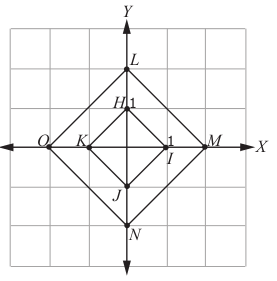
\includegraphics[scale=0.45]{Images/plano.png}
\end{center}
\begin{choices}
  \choice igual a la longitud del segmento $ \overline{HI} $
  \CorrectChoice dos veces la longitud del segmento $ \overline{HI} $
  \choice tres veces la longitud del segmento $ \overline{HI} $
  \choice cuatro veces la longitud del segmento $ \overline{HI} $
\end{choices}
\question ¿Cuáles son las coordenadas del punto $ I $? 
 
  \begin{oneparchoices}
  \choice $ (-1,0) $ \choice $ (0,-1) $ \choice $ (0,1) $ \CorrectChoice $ (1,0) $  
  \end{oneparchoices}
\question Se efectuó una traslación al cuadrilátero $ HIJK $ y el vértice $ K $ quedó en el punto de coordenadas $ (2,0) $. El cuadrilátero $ HIJK $ se trasladó \label{q02}
\begin{choices}
  \choice una unidad hacia la derecha
  \choice dos unidades hacia la derecha
  \CorrectChoice tres unidades hacia la derecha
  \choice cuatro unidades hacia la derecha
\end{choices}
\question Un rectángulo tiene 5,97 metros de largo y 8 metros de ancho. ¿Cuál de los siguientes valores es más cercano al área de este rectángulo?
\begin{choices}
\choice 40 $m^{2}$
\choice 46 $m^{2}$
\CorrectChoice 48 $m^{2}$
\choice 50 $m^{2}$
\end{choices}
\question Observa los cuadriláteros 1 y 2 dibujados en la siguiente cuadrícula:
\begin{center}
\begin{tikzpicture}[scale=.55]
\draw[dashed,style=help lines] (0,0) grid (10,4);
\draw (1,1)--(3,1)--(3,2)--(2,2)--cycle;
\node at (2,2.5) {cuadrilátero 1};
\draw (5,1)--(9,1)--(7,3)--(5,3)--cycle;
\node at (6,3.5){Cuadrilátero 2};
\end{tikzpicture}
\end{center}
Los cuadriláteros son semejantes porque
\begin{choices}
\choice tienen el mismo perímetro pero sus áreas son iguales
\choice tienen el mismo perímetro y sus áreas son diferentes
\choice sus lados correspondientes son congruentes y sus ángulos correspondientes son proporcionales
\CorrectChoice sus ángulos correspondientes son congruentes y sus lados correspondientes son proporcionales
\end{choices}
\question Observa la secuencia de figuras que se muestran a continuación.
\begin{center}
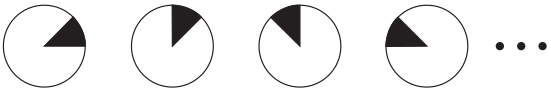
\includegraphics[scale=.30]{Images/Pantallazo-28.png} 
\end{center}
¿Cuál es la figura que sigue en la secuencia?

\begin{oneparchoices}
\choice 
\includegraphics[scale=.3]{Images/Pantallazo-29.png} 
\choice 
\includegraphics[scale=.3]{Images/Pantallazo-30.png} 
\CorrectChoice 
\includegraphics[scale=.3]{Images/Pantallazo-31.png} 
\choice 
\includegraphics[scale=.3]{Images/Pantallazo-32.png} 
\end{oneparchoices}
\question El policubo de Soma es un rompecabezas tridimensional de siete piezas, con las cuales se arma un cubo. Las siguientes figuras representan las piezas de este rompecabezas.
\begin{center}
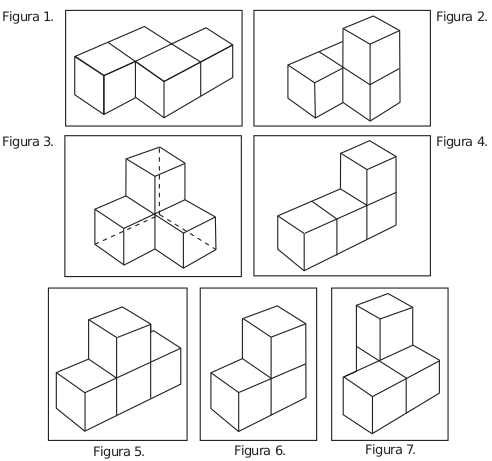
\includegraphics[scale=.3]{Images/Pantallazo-33.png} 
\end{center}
Todas las piezas se construyeron con cubos del mismo tamaño.

¿Cuál de las piezas del rompecabezas tiene menor volumen?

\begin{oneparchoices}
\choice La 1
\choice La 3
\choice La 4
\CorrectChoice La 6
\end{oneparchoices}
\question Un juguete para niños tiene tres piezas con las cuales se puede armar la siguiente figura.
\begin{center}
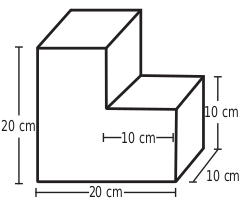
\includegraphics[scale=.3]{Images/Pantallazo-34.png} 
\end{center}
Los volúmenes de las tres piezas utilizadas para armar el sólido pueden ser:
\begin{choices}
\CorrectChoice 1000 cm$^{3}$, 1000 cm$^{3}$ y 1000 cm$^{3}$
\choice 1000 cm$^{3}$, 3000 cm$^{3}$ y 4000 cm$^{3}$
\choice 2000 cm$^{3}$, 2000 cm$^{3}$ y 2000 cm$^{3}$
\choice 2000 cm$^{3}$, 3000 cm$^{3}$ y 4000 cm$^{3}$
\end{choices}
\question Observa las siguientes figuras.
\begin{center}
\begin{tikzpicture}[scale=.35]
\draw[dashed,style=help lines] (0,0)grid (10,10);
\filldraw[gray] (0,7.5)--(0,9)--(3,9)--(3,6)--cycle;
\node at (1.5,9.5){I};
\filldraw[gray] (5,8)--(7,9)--(9,8)--(10,6)--(7,6)--cycle;
\node at (7.5,9.5){II};
\filldraw[gray] (4,1)--(4,3)--(6,4)--(8,2)--(5,0)--cycle;
\node at (5.5,4.5){III};
\end{tikzpicture}
\end{center}
¿Cuál(es) de la(s) figura(s) tiene(n) al menos un par de lados paralelos?
\begin{choices}
\choice I solamente
\choice II solamente
\CorrectChoice I y III solamente
\choice II y III solamente
\end{choices}
%\answerline
\question Los siguientes son desarrollos planos de algunos poliedros regulares.
\begin{center}
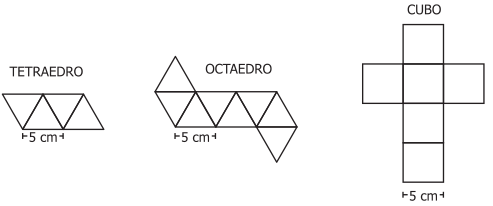
\includegraphics[scale=.3]{Images/Pantallazo-35.png}
\end{center}
Acerca del volumen de los poliedros regulares mostrados en los desarrollos anteriores, es correcto afirmar que
\begin{choices}
\choice el tetraedro tiene el mayor volumen
\choice el octaedro tiene el mayor volumen
\CorrectChoice el cubo tiene el mayor volumen
\choice todos tienen el mismo volumen
\end{choices}
%cuadro de puntajes
%\begin{center}
%\gradetable[h][pages]
%\end{center}
\question Una compañía desea construir un edificio en un terreno de forma rectangular que tiene 3.000 m$^{2}$ de área.

Las medidas de los lados del terreno pueden ser
\begin{choices}
\CorrectChoice 100 m y 30 m
\choice 100 m y 200 m
\choice 1000 m y 2000 m
\choice 1500 m y 1500 m
\end{choices}
\question Una máquina corta moldes de cartón que se doblan y se pegan para construir cajas, con las medidas que se muestran en el siguiente dibujo.
\begin{center}
\begin{tikzpicture}[scale=.7]
\draw (0,0) rectangle (2,4);
\draw (-1,2) rectangle (3,3);
\draw (0,1)--(2,1);
\node[left] at (-1,2.5){10 cm};
\node[below] at (-.5,2){10 cm};
\node[below] at (1,0){20 cm};
\node[right] at (2,1.5){10 cm};
\draw[|-] (2.25,1)--(2.25,1.25);
\draw[|-] (2.25,2)--(2.25,1.75);
\end{tikzpicture}
\end{center}
¿Cuál de las siguientes cajas se arma con el molde del dibujo?
\begin{choices}
\choice 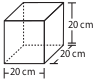
\includegraphics[scale=.35]{Images/Pantallazo-36.png} 
\CorrectChoice 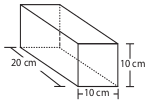
\includegraphics[scale=.35]{Images/Pantallazo-37.png} 
\choice 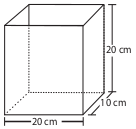
\includegraphics[scale=.35]{Images/Pantallazo-38.png} 
\choice 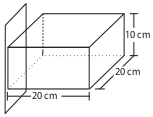
\includegraphics[scale=.35]{Images/Pantallazo-39.png} 
\end{choices}
\question En un juego Juan lanzó tres dardos a un tablero como el siguiente:
\begin{center}
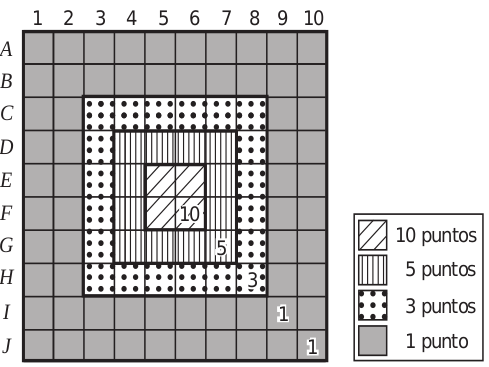
\includegraphics[scale=.3]{Images/juego_dados.png} 
\end{center}
El puntaje del juego se obtiene sumando los puntos asignados a la posición donde cae cada dardo.

Los tres dardos que lanzó Juan quedaron ubicados en los recuadros E5, F6 y D7.

¿Qué puntaje obtuvo Juan?

\begin{oneparchoices}
\choice 15 puntos
\choice 18 puntos
\choice 20 puntos
\CorrectChoice 25 puntos
\end{oneparchoices}
\question La siguiente tabla muestra los nombres de los atletas de un equipo y sus respectivos pesos
\begin{center}
\begin{tabular}[scale=.75]{|c|c|}
\hline 
\textbf{Nombre atleta} & \textbf{Peso kg} \\ 
\hline 
Oscar & 60 \\ 
\hline 
Andrés & 62.5 \\ 
\hline 
Víctor & 58.6 \\ 
\hline 
Fernando & 61.3 \\ 
\hline 
César & 65.2 \\ 
\hline 
Héctor & 59.4 \\ 
\hline 
\end{tabular} 
\end{center}
El equipo realiza algunos ejercicios en parejas. La diferencia de pesos entre los atletas que conforman una pareja no debe sobrepasar los 3 kilogramos.

¿Cuáles de los siguientes atletas del equipo no pueden realizar los ejercicios en pareja?
\begin{choices}
\choice \small Oscar y Víctor
\choice Fernando y Héctor
\CorrectChoice César y Víctor
\choice Andrés y Fernando
\end{choices}
\question En un almacén deportivo quieren empacar balones de 10 centímetros de radio en cajas cúbicas. Disponen de los siguientes moldes para armar las cajas
\begin{center}
\begin{tikzpicture}[scale=.4]
\node[above] at (0.5,4){Molde 1};
\draw (-1,1) rectangle (3,2);
\draw (0,0) rectangle (1,3);
\draw (2,1)--(2,2);
\node[scale=.75,left] at (-1,1.5){10 cm};
\node[scale=.75,above] at (0.5,3){10 cm};
\node[above] at (5.5,4){Molde 2};
\draw (4,1) rectangle (8,2);
\draw (5,0) rectangle (6,3);
\draw (6,1)--(6,2);
\node[scale=.75,right] at (8,1.5){5 cm};
\node[scale=.75,above] at (5.5,3){5 cm};
\draw (7,1)--(7,2);
\end{tikzpicture}

\begin{tikzpicture}[scale=.4]
\node[above] at (0.5,4){Molde 3};
\draw (-1,1) rectangle (3,2);
\draw (0,0) rectangle (1,3);
\draw (2,1)--(2,2);
\node[scale=.75,left] at (-1,1.5){20 cm};
\node[scale=.75,above] at (0.5,3){20 cm};
\node[above] at (5.5,4){Molde 4};
\draw (4,1) rectangle (8,2);
\draw (5,0) rectangle (6,3);
\draw (6,1)--(6,2);
\node[scale=.75,right] at (8,1.5){15 cm};
\node[scale=.75,above] at (5.5,3){15 cm};
\draw (7,1)--(7,2);
\end{tikzpicture}
\end{center}
\question En el plano cartesiano se ubican tres parejas ordenadas que son vértices de un paralelogramo.
\begin{center}
\begin{tikzpicture}[scale=.35]
\draw[dotted,style=help lines] (-.25,-2.25) grid (14.25,2.25);
\draw[<->] (-.25,0)--(14.25,0);
\foreach \x in {1,2,...,14} \draw[shift={(\x,0)},color=black] (0pt,2pt) -- (0pt,-2pt) node[below] {\footnotesize $\x$};
\draw[<->](0,-2.25)--(0,2.25);
\foreach \y in {-2,-1,1,2} \draw[shift={(0,\y)},color=black] (2pt,0)--(-2pt,0) node[left]{\footnotesize $\y$};
\filldraw (2,-2) circle (3pt) node[scale=.75,below]{(2,-2)};
\filldraw (5,1) circle (3pt) node[scale=.75,above]{(5,1)};
\filldraw (11,-2) circle (3pt) node[scale=.75,below]{(11,-2)};
\end{tikzpicture}
\end{center}
\small ¿Cuál de las siguientes parejas ordenadas puede corresponder al cuarto vértice del paralelogramo?

\begin{oneparchoices}
\choice (--3,--1)
\choice (5,--2)
\choice (11,1)
\CorrectChoice (14,1)
\end{oneparchoices}
\question \small A continuación, se enuncian propiedades de algunos cuadriláteros
\begin{itemize}
\item \small Un paralelogramo es un cuadrilátero que tiene sus lados opuestos paralelos
\item Un rombo es un paralelogramo que tiene sus 4 lados congruentes
\item Un rectángulo es un paralelogramo que tiene sus 4 ángulos rectos
\item Un cuadrado es un paralelogramo que tiene sus 4 lados congruentes y sus 4 ángulos rectos  
\end{itemize}
Observa el cuadrilátero FGHI.
\begin{center}
\begin{tikzpicture}[rotate=15,scale=.75]
\draw (0,0)rectangle (1,2);
\node[scale=.75,below] at (0,0){F};
\node[below,scale=.75] at (1,0){G};
\node[above,scale=.75] at (1,2){H};
\node[above,scale=.75] at (0,2){I};
\draw (.15,0)--(.15,.15)--(0,.15);
\draw (.85,0)--(.85,.15)--(1,.15);
\draw (1,1.85)--(.85,1.85)--(.85,2);
\draw (0,1.85)--(0.15,1.85)--(.15,2);
\end{tikzpicture}
\end{center}
El cuadrilátero FGHI de la figura es
\begin{choices}
\choice un rombo pero no un cuadrado
\CorrectChoice un rectángulo pero no un rombo
\choice un paralelogramo
\choice un cuadrado
\end{choices}
\end{questions}
\end{multicols}
\end{document}